\documentclass[a4paper,
fontsize=11pt,
%headings=small,
oneside,
numbers=noperiodatend,
parskip=half-,
bibliography=totoc,
final
]{scrartcl}

\usepackage[babel]{csquotes}
\usepackage{synttree}
\usepackage{graphicx}
\setkeys{Gin}{width=.7\textwidth} %default pics size

\graphicspath{{./plots/}}
\usepackage[ngerman]{babel}
\usepackage[T1]{fontenc}
%\usepackage{amsmath}
\usepackage[utf8x]{inputenc}
\usepackage [hyphens]{url}
\usepackage{booktabs} 
\usepackage[left=2.4cm,right=2.4cm,top=2.3cm,bottom=2cm,includeheadfoot]{geometry}
\usepackage[labelformat=empty]{caption} % option 'labelformat=empty]' to surpress adding "Abbildung 1:" or "Figure 1" before each caption / use parameter '\captionsetup{labelformat=empty}' instead to change this for just one caption
\usepackage{eurosym}
\usepackage{multirow}
\usepackage[ngerman]{varioref}
\setcapindent{1em}
\renewcommand{\labelitemi}{--}
\usepackage{paralist}
\usepackage{pdfpages}
\usepackage{lscape}
\usepackage{float}
\usepackage{acronym}
\usepackage{eurosym}
\usepackage{longtable,lscape}
\usepackage{mathpazo}
\usepackage[normalem]{ulem} %emphasize weiterhin kursiv
\usepackage[flushmargin,ragged]{footmisc} % left align footnote
\usepackage{ccicons} 
\setcapindent{0pt} % no indentation in captions

%%%% fancy LIBREAS URL color 
\usepackage{xcolor}
\definecolor{libreas}{RGB}{112,0,0}

\usepackage{listings}

\urlstyle{same}  % don't use monospace font for urls

\usepackage[fleqn]{amsmath}

%adjust fontsize for part

\usepackage{sectsty}
\partfont{\large}

%Das BibTeX-Zeichen mit \BibTeX setzen:
\def\symbol#1{\char #1\relax}
\def\bsl{{\tt\symbol{'134}}}
\def\BibTeX{{\rm B\kern-.05em{\sc i\kern-.025em b}\kern-.08em
    T\kern-.1667em\lower.7ex\hbox{E}\kern-.125emX}}

\usepackage{fancyhdr}
\fancyhf{}
\pagestyle{fancyplain}
\fancyhead[R]{\thepage}

% make sure bookmarks are created eventough sections are not numbered!
% uncommend if sections are numbered (bookmarks created by default)
\makeatletter
\renewcommand\@seccntformat[1]{}
\makeatother

% typo setup
\clubpenalty = 10000
\widowpenalty = 10000
\displaywidowpenalty = 10000

\usepackage{hyperxmp}
\usepackage[colorlinks, linkcolor=black,citecolor=black, urlcolor=libreas,
breaklinks= true,bookmarks=true,bookmarksopen=true]{hyperref}
\usepackage{breakurl}

%meta
%meta

\fancyhead[L]{K. Schuldt\\ %author
LIBREAS. Library Ideas, 43 (2023). % journal, issue, volume.
\href{https://doi.org/10.18452/...}{\color{black}https://doi.org/10.18452/...}
{}} % doi
\fancyhead[R]{\thepage} %page number
\fancyfoot[L] {\ccLogo \ccAttribution\ \href{https://creativecommons.org/licenses/by/4.0/}{\color{black}Creative Commons BY 4.0}}  %licence
\fancyfoot[R] {ISSN: 1860-7950}

\title{\LARGE{Werden die Öffentlichen Bibliotheken von zwei unterschiedlichen Gruppen benutzt? Ein konzeptionelles Modell}}% title
\author{Karsten Schuldt} % author

\setcounter{page}{1}

\hypersetup{%
      pdftitle={Werden die Öffentlichen Bibliotheken von zwei unterschiedlichen Gruppen benutzt? Ein konzeptionelles Modell},
      pdfauthor={Karsten Schuldt},
      pdfcopyright={CC BY 4.0 International},
      pdfsubject={LIBREAS. Library Ideas, 43 (2023).},
      pdfkeywords={Öffentliche Bibliothek, Bibliotheksnutzung, Raum, Bestand},
      pdflicenseurl={https://creativecommons.org/licenses/by/4.0/},
      pdfurl={https://doi.org/10.18452/...},
      pdfdoi={10.18452/...},
      pdflang={de},
      pdfmetalang={de}
     }



\date{}
\begin{document}

\maketitle
\thispagestyle{fancyplain} 

%abstracts
\begin{abstract}
\noindent
\textbf{Kurzfassung}: Anhand eines Beispiels zeigt der Artikel, welche
Konsequenzen ein soziologisch orientiertes Denken für die
Bibliothekspraxis haben könnte. Es wird eine These über die Nutzung
Öffentlicher Bibliotheken entwickelt, Evidenzen für diese gesammelt und
anschliessend ein konzeptionelles Modell erstellt, mit dem diese These
überprüft werden kann. Es wird postuliert, dass es sei unterschiedliche
Gruppen von Nutzer*innen gibt, eine bestandsbezogene und eine
raumbezogene. Zusätzlich wird diskutiert, welche Konsequenzen für die
Praxis Öffentlicher Bibliotheken gezogen werden könnten, wenn sich die
These als richtig herausstellt.

\begin{center}\rule{0.5\linewidth}{0.5pt}\end{center}

\textbf{Abstract}: Using an example, the article shows what consequences
sociologically-oriented thinking could have for library practice. It
develops a thesis about the use of public libraries, collects evidence
for it and creates a conceptual model with which this thesis can be
tested. It is postulated that there are different groups of users, one
collection-related and one space-related. In addition, it discusses
possible consequences for the practice of public libraries if the thesis
proves to be correct.
\end{abstract}

%body
Soziologie, so der Call for Paper für diese Ausgabe der LIBREAS. Library
Ideas (Redaktion LIBREAS 2022), fragt danach, wie die Gesellschaft
funktioniert, also zum Beispiel wie das Handeln unterschiedlicher
Individuen dazu führt, dass Institutionen funktionieren oder
gesellschaftliche Strukturen reproduziert werden. Von einem solchen
Wissen können die betreffenden Institutionen profitieren, weil so zum
Beispiel verständlicher wird, warum die Institution so genutzt wird, wie
sie es jeweils wird oder auch, weil Zielsetzungen der Institutionen
realistisch gesteckt werden können. Sicherlich ist dafür dann eine
Transformation des Wissens notwendig: Aus dem in der Forschung
produzierten Wissen darüber, wie gesellschaftliche Strukturen sich im
Handeln einzelner Individuen niederschlagen, müssen von der jeweiligen
Institution Schlüsse gezogen und dann umgesetzt werden, um wirksam zu
werden. Diese Transformation ist nicht Thema des vorliegenden Textes.
Vielmehr wird sich hier auf den ersten Aspekt fokussiert, nämlich dem
Thema, wie die Nutzung einer Institution -- die Öffentliche Bibliothek
-- funktioniert. Dabei wird hier auch nicht von einer durchgeführten
Studie oder empirischen Daten berichtet -- sondern von einem Schritt vor
einer solchen Studie. Aus Beobachtungen über die Nutzung der
Öffentlichen Bibliotheken wird ein konzeptionelles Modell über diese
Nutzung erstellt. Dieses Modell kann dann in Zukunft forschend
widerlegt, bestätigt oder auch angepasst werden.

Der Text versteht sich unter anderem als Test dafür, ob es möglich ist,
Überlegungen zur Nutzung der Öffentlichen Bibliotheken in ein solches
Modell zu fassen. Und gleichzeitig als Nachweis darüber, dass eine
solche Systematisierung zu Wissen führen kann, welches für die Praxis
Öffentlicher Bibliotheken Relevanz hat. Er ist in gewisser Weise auch
als Aufruf an andere zu verstehen, sich solchen Systematisierungen zu
widmen.

Aufgebaut ist der Text wie folgt: Im ersten Kapitel (1.) wird die These
genannt und anschliessend (Kapitel 2.) Evidenzen dafür versammelt,
welche diese These stützen. Daraufhin (Kapitel 3.) wird diskutiert,
welche Konsequenzen sich für die Bibliothekspraxis ergeben könnten, wenn
sich die These als richtig herausstellt. Dieses Kapitel hat hier die
Aufgabe, zu zeigen, dass ein soziologisch orientiertes Nachdenken
darüber, wie Bibliotheken funktionieren, nicht praxisfern wäre. Kapitel
4. wird dann ein konzeptionelles Modell präsentieren, welches die These
und die vorhergehend diskutierten Evidenzen so strukturiert, dass sich
daraus Vorhersagen ziehen lassen, welche empirisch überprüft werden
können und damit die These entweder falsifizieren und stützen. Vor dem
Fazit (Kapitel 6.) wird in Kapitel 5. noch ein potentielles
Forschungsprogramm, welches sich auf das konzeptionelle Modell stützt,
entworfen. Dieses soll am Beispiel der hier besprochenen These zeigen,
wie eine soziologisch aufgebaute Forschung über Bibliotheken organisiert
werden kann.

\hypertarget{these-von-den-zwei-gruppen}{%
\section{1. These von den zwei
Gruppen}\label{these-von-den-zwei-gruppen}}

Die These, welche in diesem Text begründet werden und für die dann
anschliessend überlegt werden soll, wie sie untersucht werden kann und
welche Konsequenzen es für Öffentliche Bibliotheken hätte, wenn sie
bestätigt würde, ist folgende:

\emph{In der Öffentlichen Bibliothek stellen die Nutzer*innen des Raumes
der Bibliothek und die Nutzer*innen der Medien zwei unterschiedliche
Gruppen dar. Die Interessen und Verhaltensweisen dieser zwei Gruppen
unterscheiden sich, auch wenn sie nicht vollständig distinkt sind und
Individuen über einen längeren Zeitraum hinweg gesehen zwischen diesen
Gruppen wechseln können.}

\hypertarget{evidenzen}{%
\section{2. Evidenzen}\label{evidenzen}}

Die genannte These steht -- darum wird es gehen, wenn weiter unten die
möglichen Konsequenzen diskutiert werden -- dem entgegen, wie im
Öffentlichen Bibliothekswesen und der dazugehörigen Literatur in den
letzten Jahren reale und potentielle Veränderungen in der Nutzung von
Bibliotheken diskutiert und wahrgenommen werden. Dort scheint es --
zumindest im DACH-Raum -- einen gewissen Konsens darüber zu geben, dass
die Nutzung von Medien, insbesondere physischer Medien, an Bedeutung
verliert, während die Nutzung des Raumes der Bibliotheken zunehmen
würde. (Vergleiche zum Beispiel die Schwerpunkte der Ausgabe 01/2022 und
05/2022 der \emph{BuB: Forum Bibliothek und Information}.) Diese oft
geäusserten Vermutungen werden selten mit Daten unterlegt, aber oft in
einer Weise berichtet, als ob klar wäre, dass diese postulierten
Entwicklungen fraglos in einem engen Zusammenhang stehen würden. Die
Nutzer*innen von Bibliotheken werden als eine zusammengehörige Gruppe
verstanden, welche insgesamt ihr Verhalten und ihre Nutzungsweisen von
Medien und Räumen ändern würde.

So sind dann beispielsweise auch Umfragen, die von Bibliotheken
durchgeführt werden, oder partizipative Projekte, mit denen über die
Weiterentwicklung von Bibliotheken entschieden werden sollen, aufgebaut.
Immer wieder scheint es, als würde -- obgleich ansonsten in der
bibliothekarischen Literatur oft von unterschiedlichen Zielgruppen
gesprochen wird -- zumindest implizit davon ausgegangen, dass sich die
Interessen von Nutzer*innen insgesamt verändern würden und als könnte
man diese deshalb als eine zusammengehörige Gruppe beschreiben. Diese
Überzeugung lässt sich implizit als These über die Nutzer*innen als
zusammengehörige Gruppe beschreiben.

Aber ein genauerer Blick auf die -- zugegeben wenigen -- vorhandenen
Daten über die tatsächliche Nutzung Öffentlichen Bibliotheken im
DACH-Raum legt zumindest eine mögliche andere Deutung nahe, aus der die
oben schon genannte These formuliert wurde.

In einer Studie aus der University of Nebraska-Lincoln, vor einigen
Jahren publiziert, aber in ihrer Relevanz offenbar nicht so richtig
erkannt, untersuchten Allison et al.~(2019), wie sich die Einrichtung
eines Learning Commons in der dortigen Universitätsbibliothek auf die
Nutzung des Bestandes und Raumes auswirkt. Dabei referierten sie zuerst,
dass sich in der Literatur zu Learning Commons und ähnlichen Umbauten
von Wissenschaftlichen Bibliotheken immer wieder Aussagen finden, die
den oben zu Öffentlichen Bibliotheken im DACH-Raum angeführten ähneln.
In dieser Literatur wird angenommen, dass es grundsätzlich weniger
Nutzung von Medien und dafür mehr Nutzung des Raumes von Bibliotheken
gäbe und daraus oft geschlossen, dass Bibliotheken recht daran tun, auf
diese Trends mit der Einrichtung von Lernzentren und dem Abbau von
physischen Medienbeständen zu reagieren. Es gibt dazu, wie Allison et
al.~(2019) angeben, auch Beiträge, die sich kritisch äussern. Aber --
und das ist der hier wichtige Punkt -- fast alle diese Beiträge zum
Thema kommen ohne Daten aus.

Was Allison et al.~(2019) in ihrer Studie dann tun, ist, solche Daten
nach der 2016 erfolgten Eröffnung der Learning Commons in Lincoln
zusammenzustellen. Das methodische Vorgehen und die genauen, sicher auch
von lokalen Bedingungen beeinflussten, Daten lassen sich im Artikel
nachvollziehen. Relevant ist hier das grundsätzliche Ergebnis: Es zeigte
sich kein Zusammenhang zwischen der Nutzung des Lernzentrums und der
Bestände. Auf der einen Seite wurden die neu eingerichteten Lern- und
Arbeitsplätze intensiv genutzt. Damit stieg auch die Zahl der gezählten
Nutzer*innen. Aber gleichzeitig veränderte sich die Nutzung der Bestände
praktisch nicht, obgleich sogar eine grosse Anzahl von Medien aus der
Bibliothek entfernt wurden. Auch die Zahl der Fernleihen zeigte keine
grosse Veränderung.

Allison et al.~(2019) schliessen nun aus ihren Daten, dass zumindest in
Lincoln zwei Gruppen von Nutzer*innen existieren: Diejenigen, welche
durch die Eröffnung der Learning Commons zu einer häufigeren Nutzung der
Bibliothek als Arbeitsort (oder zumindest als Aufenthaltsort, die
konkrete Tätigkeit wurde nicht gemessen) gebracht werden. Und
diejenigen, welche die Medien nutzen und sich dabei (zumindest im
Zeitraum, für den Daten gesammelt wurden) nicht durch die Einrichtung
der Learning Commons und den Abbau der physischen Bestände erkennbar
beeinflussen lassen.

Sicherlich ist diese Studie von Allison et al.~(2019) nicht einfach
übertragbar. Sie bezieht sich auf eine Wissenschaftliche Bibliothek in
den USA, nicht auf Öffentliche Bibliotheken im DACH-Raum. Zudem ist es
genau eine Studie, bei der naturgemäss nicht einfach geklärt werden
kann, welchen Einfluss die lokalen Gegebenheiten auf die Daten haben
oder, umgekehrt, wie sehr diese Daten verallgemeinert werden können. Was
die Studie trotzdem zeigt, ist, dass es sich lohnt, sich danach zu
fragen, ob und, wenn ja, wie Veränderungen in der Nutzung des Raumes von
Bibliotheken mit Veränderungen der Nutzung des Bestandes zusammenhängen.
Grundsätzlich zeigte sie ja für die Bibliothek in Lincoln, dass die
Entscheidung, einen Teil des physischen Bestandes aus dem
Bibliotheksraum zu entfernen und ein Lernzentrum einzurichten, eine
produktive Entscheidung war, die zu einer insgesamt höheren
Bibliotheksnutzung führte, aber in einer anderen Weise, als man das auf
Basis der bibliothekarischen Fachliteratur hätte erwarten können.

Eine weitere Evidenz dafür liefert ein aktueller Artikel von Lori Cisney
(2023). In diesem wird -- für Medizinbliotheken in den USA -- von einer
Studie berichtet, in der danach gefragt wurde, ob die
Bibliothekar*innen, welche in den befragten Bibliotheken für die
Veranstaltungen zur Informationskompetenz zuständig sind, und die
Bibliothekar*innen, welche in den gleichen Bibliotheken Aufgaben im
Bereich des Bestandsmanagements übernehmen, ihre Arbeit aufeinander
abstimmen. Cisney (2023) zeigt, dass dies fast nicht passiert, sondern
dass in der Praxis Veranstaltungs- und Beratungsarbeit auf der einen
Seite und Bestandsmanagement auf der anderen Seite relativ losgelöst
voneinander betrieben werden. Dies kann man als problematisch ansehen,
wenn man davon ausgeht, dass die Arbeit einer Bibliothek möglichst eng
koordiniert sein sollte, also in diesem Falle, dass im
Bestandsmanagement darauf geachtet werden sollte, Medien zu erwerben,
die mit dem übereinstimmen, was in den Veranstaltungen zu
Informationskompetenz thematisiert wird. Eine alternative Deutung ist
aber auch möglich: Eventuell zeigt sich hier eine Praxis, die sich im
Alltag der Bibliotheken als sinnvoll und effizient etabliert hat, weil
die beiden Bereiche -- auf der einen Seite Veranstaltungen, auf der
anderen der Bestand -- sich an verschiedene Gruppen von Nutzer*innen
richten, die unterschiedliche Erwartungen haben und in der Bibliothek
auch unterschiedliche Dinge tun. Eine enge Koordination der
Aufgabenbereiche in der Bibliothek würde dann Sinn machen, wenn es sich
um die gleiche Gruppe von Nutzer*innen handeln würde, also wenn diese
das, was sie in den Veranstaltungen zur Informationskompetenz lernen,
auch bei der Nutzung der Medien verwenden würden. Aber wenn das nicht
der Fall ist, dann kann eine Koordination in der Praxis auch eine
unnötige, eventuell auch ineffiziente Arbeit darstellen.

Im DACH-Raum werden Bibliotheksstatistiken geführt, in denen ebenso
Ausschau nach Evidenzen dafür gehalten werden kann, ob es Parallelen zu
den von Allison et al.~(2019) festgestellten unterschiedlichen
Nutzungsgruppen gibt. Hierzu verwende ich Daten, die ich für eine andere
Fragestellung schon einmal ausgewertet habe. (Schuldt 2022) Die Daten
beziehen sich aufgrund der originalen Fragestellung auf Öffentliche
Bibliotheken und stammen aus den Bibliotheksstatistiken aus Deutschland,
Österreich und der Schweiz für die Jahre 2018--2020. Sie stellen also
nicht mehr die jeweils neusten Daten dar. Ich verwende sie trotzdem, da
in Ihnen meiner Meinung nach schon bei der ersten Auswertung eine
ähnliche Dynamik sichtbar wurde, wie sie Allison et al.~(2019) gefunden
haben.

Im Artikel, für den ich die Daten zuerst versammelt habe, wurde danach
gefragt, ob die Covid-19 Pandemie einen krisenhaften Einfluss auf die
Öffentlichen Bibliotheken im DACH-Raum hatte. Ausgangspunkt war eine
Arbeit, die eine solche Krise für die Public Libraries in
Grossbritannien zeigte. (McMenemy et al.~2023) Für den DACH-Raum liess
sich eine solche Entwicklung nicht nachweisen. Vielmehr zeigten hier die
Öffentlichen Bibliotheken relativ stabile Nutzungszahlen, zumindest über
alle Bibliotheken hinweg gemessen, wenn auch mit nationalen
Unterschieden. Als Beispiel sei folgende Tabelle (Tabelle 1) zu den
aktiven Nutzer*innen (also denen, die im jeweils angegebenen Jahr
mindestens ein Medium aus einer Bibliothek entliehen haben) angeführt.
Praktisch die gleichen Entwicklungen zeigen sich auch bei der
Medienausleihe.

\begin{table}
\begin{center}
\begin{tabular}{lrrr}
Land & 2018 & 2019 & 2020 \\ 
 \hline
Deutschland & 7.076.280 & 7.141.002 & 6.307.585 \\
Österreich & 798.109 & 813.074 & 755.220 \\
Schweiz & 890.919 & 835.941 & 897.591 \\
\end{tabular}
\caption{Tabelle 1: Anzahl aktive Nutzer*innen, 2018--2020}
\end{center}
\end{table}

Der Bereich, in dem sich diese Entwicklung nicht zeigt, ist die Zahl der
aktiven Besuche. Hier, dargestellt in Tabelle 2, zeigt sich ein
expliziter Einbruch der Zahlen, der wohl auf die Verhaltensänderungen
von Menschen und die von den Behörden erlassenen Beschränkungen während
der Frühphase der Covid-19 Pandemie zurückgeführt werden können.

\begin{table}
\begin{center}
\begin{tabular}{lrrr}
Land & 2018 & 2019 & 2020 \\
\hline
Deutschland & 112.602.769 & 114.850.449 & 69.236.498 \\
Österreich & 10.250.026 & 10.422.581 & 7.115.664 \\
Schweiz & 9.890.886 & 10.324.575 & 8.071.941 \\
\end{tabular}
\caption{Tabelle 2: Anzahl Besuche, 2018--2020}
\end{center}
\end{table}

Eine Deutung dieser Zahlen wäre, sie grundsätzlich auf die Covid-19
Pandemie zurückzuführen: Menschen hätten einerseits mehr Zeit gehabt,
Medien zu konsumieren und gleichzeitig weniger Möglichkeiten,
Bibliotheken vor Ort zu nutzen.

Aber es ist auch eine alternative Deutung möglich, welche eher zur oben
genannten These passt. Eventuell zeigen diese Zahlen die
Verhaltensänderung verschiedener Gruppen, welche von der Pandemie und
den Massnahmen gegen ihre Verbreitung erzwungen waren. In dieser
alternativen Deutung zeigt sich in der einen bestandsbezogenen Gruppe,
welche vor allem Medien aus Bibliotheken ausleiht (und dann wohl nutzt),
dass sie dies auch 2020 stark taten und in der anderen ortsbezogenen
Gruppe, dass sie 2020 die Bibliotheken weniger nutzten. Sicherlich: So
wie in den Bibliotheksstatistiken Besuche gezählt werden (also als
jeweils ein Eintritt in die Bibliothek, im Idealfall durch einen Zähler
am Eingang festgehalten), finden sich in den Zahlen zu den Besuchen
immer alle Personen, die die Bibliothek betreten, egal zu welchem Zweck
und egal für wie lange. Also immer auch die, welche die Bibliothek nur
zur Rückgabe und Ausleihe von Medien nutzen.\footnote{Aber
  selbstverständlich nicht die, welche nur die elektronischen Angebote
  von Bibliotheken nutzen. Wie die Auswertung der vorhandenen --
  allerdings für elektronische Medien nicht vollständigen -- Daten
  zeigte, ist diese Nutzung aber weiterhin, wenn auch nicht unbedeutend,
  so doch nicht die Hauptnutzungsart von Öffentlichen Bibliotheken. Die
  Ausleihe physischer Medien ist weiterhin wichtiger.} Aber die Daten
können dennoch dahingehend gedeutet werden, dass sie vor allem die
geringe Nutzung durch die Gruppe von Personen, welche die Bibliothek vor
allem als Ort nutzen, andeuten.

Ein letzter Punkt sei als zumindest schwache Evidenz noch angeführt: In
Öffentlichen Bibliotheken gibt es seit Jahrzehnten Überlegungen, immer
wieder neue Angebote einzuführen. Makerspaces, Debatten um den «Dritten
Ort» oder die Bibliothek als «Zentrum des Dorfes» sind da nur die
letzten in einer langen Reihe von jeweils neuen Angeboten. Insbesondere
am Anfang der jeweiligen Zyklen, wenn diese Angebote tatsächlich für das
Bibliothekswesen noch recht neu sind, gibt es wohl immer wieder die
Hoffnung, mit diesen auch die Nutzung «traditioneller Angebote» -- womit
zumeist die Ausleihe physischer Medien gemeint ist -- zu erhöhen.
Nachdem die Angebote dann relativ normal geworden sind, werden diese
kaum noch mit diesen «traditionellen Angeboten» in Verbindung gebracht.
Dafür kann es verschiedene Gründe geben, aber es drängt sich die
Vermutung auf, dass dieser erhoffte Zusammenhang einfach in der Realität
kaum zu beobachten ist.\footnote{Ein herausgegriffenes Beispiel dafür
  ist das Thema Spiele (sowohl Computer- und Konsolengames als auch
  Brettspiele) in Public Libraries. Anfang der 2010er Jahre wurde dieses
  Thema in den USA regelrecht kampagnenartig als mögliches Angebot
  beworben. Scott Nicholson -- der damals das heute eingestellte
  «Library Game Lab» an der Syracuse University, New York betreute --
  schrieb zum Beispiel in der Einleitung zu seinem Buch «Everyone plays
  at the library» explizit ein Kapitel zu der Frage, «What Do Games Have
  to Do With Books?» (Nicholson 2010: 5--12), in welchem er den
  Zusammenhang von Spielen und Lesen benannte. In der drei Jahre später
  von ihm herausgegebenen Schwerpunktnummer der Zeitschrift
  \emph{Library Trends} zu «The Impact of Gaming on Libraries»
  (Nicholson 2013) kommt diese Verbindung praktisch nicht mehr vor,
  obwohl sie bei dem Schwerpunkttitel eigentlich zu erwarten wäre.
  Heute, wo Spiele als Angebot von Public Libraries in den USA etabliert
  sind, kommen betreffende Handbücher (siehe zum Beispiel Kroski 2020)
  praktisch ohne Erwähnung der «traditionellen Angebote» aus.} Eine
mögliche Erklärung dafür wäre, dass es sich wieder nicht um eine Gruppe
von Nutzer*innen handelt, sondern dass die Personen, welche von den
jeweils «neuen Angeboten» angesprochen werden, eine andere Gruppe
darstellen, als die, welche physische Medien entleihen -- und zwar immer
wieder so distinkt, dass es auch nach der Etablierung der jeweiligen
neuen Angebote nicht zu nennenswerten Überschneidungen kommt. Ob das so
ist, liesse sich selbstverständlich nur klären, wenn man dies explizit
untersucht. Aber solche Untersuchungen scheint es praktisch nicht zu
geben. Sie müssten erst geplant werden und dazu auch einem
konzeptionellen Modell folgen -- wie dem, welches im vorliegenden
Artikel erst skizziert werden soll.

Es geht also auch um einen gewissen Zirkelschluss: Die notwendigen
Untersuchungen, um die oben genannte These zu testen, existieren nicht,
weil die These selbst nicht verbreitet ist. Dabei hätte die These, wenn
sie bestätigt würde, möglicherweise eine Anzahl von Konsequenzen für die
Bibliothekspraxis. Um diese soll es im nächsten Kapitel gehen, bevor
dann im darauffolgenden endlich das angedeutete Modell für potentielle
Untersuchungen der These erstellt wird.

\hypertarget{muxf6gliche-konsequenzen}{%
\section{3. Mögliche
Konsequenzen}\label{muxf6gliche-konsequenzen}}

Die oben aufgestellte These hätte, wenn sie sich als korrekt
herausstellen würde, einige Konsequenzen für die Arbeit und strategische
Planung von Öffentlichen Bibliotheken. Selbstverständlich müssten diese
Konsequenzen von den Bibliotheken und deren Leitungen selbst gezogen
werden. Untersuchungen können für solche Entscheidungen immer nur Daten
und Argumente liefern. Aber -- und deshalb soll hier einmal genauer
darauf eingegangen werden -- die hier präsentierte These ist ein gutes
Beispiel dafür, welche Auswirkungen soziologisch orientiertes Denken auf
die Bibliothekspraxis haben könnte.

\begin{enumerate}
\def\labelenumi{\arabic{enumi}.}
\item
  Grundsätzlich würde es bedeuten, dass bei strategischen Planungen
  andere Schwerpunkte gesetzt werden sollten. Bisherige
  Bibliotheksstrategien fokussieren oft darauf, was an Bibliotheken und
  deren Angeboten verändert werden sollte.\footnote{Die meisten
    Bibliotheksstrategien werden nicht veröffentlicht, insoweit ist
    diese Aussage schwer empirisch zu bestätigen. Allerdings ist der
    Autor im Rahmen seiner Arbeit immer wieder in unterschiedlichen
    Rollen in Strategieprozessen von Bibliotheken verschiedener Grössen
    eingebunden und denkt deshalb, diese grobe Aussage machen zu können.}
  Im Mittelpunkt stehen wohl oft Neuentwicklungen, Um- und Neubauten
  oder neue Aufgaben für das Bibliothekspersonal, die vor allem darauf
  zielen, neue Angebote -- zumindest für die konkrete Bibliothek --
  aufzubauen. Seltener geht es um eine andere, effektivere Gestaltung
  der schon getätigten Arbeit, aber auch dann zumeist mit dem Ziel, neue
  Angebote zu ermöglichen. Die meisten dieser neuen Angebote zielen nun
  darauf ab, neue oder erweiterte Nutzungen des Bibliotheksraumes zu
  ermöglichen, ob mit Makerspaces, Bibliothekscafés, Urban Gardens,
  Lernzentren oder auch erweiterten Öffnungszeiten. Falls sich die These
  von den zwei Gruppen als korrekt herausstellt, würde damit aber nur
  eine Gruppe angesprochen und die zweite Gruppe mehr oder minder
  übersehen.
\item
  Sollte sich tatsächlich zeigen, dass zwei Gruppen -- eine
  bestandsbezogene und eine raumbezogene -- Öffentliche Bibliotheken
  stark nutzen, dann würde das die Bedeutung des Bestandsmanagements
  verändern gegenüber dem Nachdenken über neue Angebote von Bibliotheken
  und der Ausgestaltung des Bibliotheksraumes. Ein kursorischer Blick in
  die Fachliteratur, welche auf das Öffentliche Bibliothekswesen zielt
  -- also vor allem die \emph{BuB: Forum Bibliothek und Information},
  die \emph{Büchereiperspektiven} und die \emph{bibliosuisse info}, die
  Zeitschriften der Börromäusverbände und des Evangelischen
  Literaturportals, aber auch die Publikationen und
  Fortbildungsprogramme von verschiedenen Fachstellen --, zeigt heute,
  dass die eigentliche Arbeit mit dem Bestand -- ausser in den
  Buchbesprechungen der konfessionell organisierten Büchereivereine --
  sehr selten thematisiert wird. Grundsätzlich sollte aber, wenn sich
  die These als richtig herausstellt, nicht nur über Angebote für die
  Gruppe der «raumbezogenen» Nutzer*innen, sondern auch der
  «bestandsbezogenen» nachgedacht werden.
\item
  Seit Beginn des 20. Jahrhunderts ist das Öffentliche Bibliothekswesen
  unter anderem damit beschäftigt, die unterschiedlichen Öffentlichen
  Bibliotheken zu differenzieren, in Gruppen einzuteilen und über die
  mögliche Zusammenarbeit unterschiedlicher Öffentlicher Bibliotheken
  nachzudenken. Die angedachten und auch umgesetzten Lösungen dazu waren
  im Laufe der Zeit sehr unterschiedlich -- beginnend bei der Akzeptanz
  von Unterschieden über die eher lose Verkoppelung von Bibliotheken,
  insbesondere durch die übergreifende Beratung von Fachstellen, bis hin
  zu streng zentralistischen Lösungen in gegliederten Netzwerken. Aber
  was sich immer wieder zeigte, war, dass Bibliotheken unterschiedlicher
  Grösse unterschiedliche Angebote machen und dass die Grösse von
  Bibliotheken in gewisser Weise von der Grösse der jeweiligen Gemeinden
  abhängt. Tendenziell haben grössere Gemeinden auch grössere
  Bibliotheken (oder in einigen Fällen grössere Bibliotheksnetze
  inklusive Zentralbibliotheken) und gleichzeitig haben grössere
  Bibliotheken ein breiteres Angebot. Gerade letzteres ist relevant,
  weil sich in der Praxis oft die Frage stellt -- und auch vor Ort in
  kleinerer Gemeinden dazu Vermutungen angestellt werden --, dass sich
  der Aufwand an Ressourcen und Zeit für bestimmte Angebote nur in
  bestimmten, grösseren Bibliotheken «lohnen» würde. Wenn sich die These
  von den zwei Gruppen bestätigen würde, dann könnte dies einen weiteren
  Faktor hinzufügen, um diesen Unterschied zu erklären. Eventuell ist
  die zweite, raumbezogene Gruppe an Nutzer*innen kleiner als die erste,
  bestandsbezogene, und es bedarf erst einer gewissen Gemeindegrösse,
  damit sich unter den Bewohner*innen der jeweiligen Gemeinde auch
  genügend potentielle Mitglieder dieser zweiten Gruppe finden, damit
  von der jeweiligen Bibliothek zum Beispiel ein Makerspace oder ein
  Urban Garden erfolgreich und kontinuierlich betrieben werden kann.
  Eine solche Frage lässt sich stellen, wenn das Vorhandensein von zwei
  Gruppen akzeptiert wird und nicht implizit den jetzigen Nutzer*innen
  unterstellt wird, sie hätten gesamthaft Interesse an raumbezogenen
  Angeboten.
\item
  Grundsätzlich liesse sich der Einsatz von Ressourcen und Personal,
  inklusive der Weiterentwicklung von Personal, besser planen, wenn klar
  wäre, ob es die beiden Gruppen aus der These gibt, wie sich deren
  Interessen verteilen und wie gross ihre Anteile sind. Es gibt Hinweise
  darauf, dass dies in der Praxis implizit auch schon teilweise gemacht
  wird. Der Einsatz von Medienpädagogik*innen in deutschen Bibliotheken,
  deren Aufgaben sich grob -- in der Unterteilung, wie sie in der These
  gemacht wird -- den raumbezogenen Angeboten zuordnen lassen, während
  Bibliothekar*innen in den betreffenden Bibliotheken eher die
  bestandsbezogenen Aufgaben wahrnehmen, liesse sich so erklären. Würde
  sich bestätigen, dass es sich um Aufgaben für zwei unterschiedliche
  Gruppen von Nutzer*innen handelt, dann müsste so ein Personaleinsatz
  nicht negativ gesehen werden, sondern könnte aktiver gesteuert werden.
\item
  Zuletzt liesse sich auch die Bewertung der Arbeit von Bibliotheken
  fairer durchführen. Bislang wird diese -- egal, ob sie anhand von
  Kennzahlen und Bibliotheksstatistiken durchgeführt wird oder verbal
  mit der Darstellung der Arbeit, beispielsweise in Jahresberichten --
  implizit unter der Prämisse vorgenommen, dass es sich bei den
  (potentiellen) Nutzer*innen von Bibliotheken um eine Gruppe handeln
  würde, deren Interesse an bestands- und raumbezogener Nutzung ungefähr
  gleich verteilt wäre. Sicherlich werden heute Unterteilungen der
  Nutzer*innenschaft anhand von Alter und -- abnehmend -- Geschlecht
  gemacht (und ohne Frage gab es während des 20. Jahrhunderts noch weit
  mehr Kriterien, nach denen die Nutzer*innenschaft unterteilt wurde,
  beispielsweise dem sozialen Stand). Was allerdings bei all diesen
  Differenzierungen beibehalten wird, ist die Vermutung, dass es keinen
  statistischen Unterschied innerhalb dieser Gruppen mit Bezug darauf
  gibt, ob sie die Bibliothek eher wegen des Bestandes oder wegen des
  Raumes nutzen. Sollte sich aber zeigen, dass es die zwei postulierten
  Gruppen gibt, dann wäre es sinnvoll, diese nicht nur bei der Planung
  des Ressourceneinsatzes von Bibliotheken zu beachten, sondern auch bei
  der Bewertung.
\end{enumerate}

\hypertarget{konzeptuelles-modell}{%
\section{4. Konzeptuelles Modell}\label{konzeptuelles-modell}}

Nach den vorausgegangenen Überlegungen wird in diesem Kapitel ein
(erstes) konzeptionelles Modell präsentiert, mithilfe dessen die
aufgestellte These überprüft werden kann. In einem solchen Modell wird
versucht, Elemente und Verbindungen, die sich aus einer These ergeben,
so darzustellen, dass Ansätze sichtbar werden, welche untersucht werden
können, um die jeweilige These widerlegen oder bestätigen zu können. Im
Idealfall ergeben sich aus einem solchen Modell Vorhersagen über
bestimmte Zusammenhänge oder Ergebnisse, die dann überprüft werden
können.

Das hier vorgestellte konzeptionelle Modell fasst zusammen, was bislang
über die beiden postulierten Gruppen gesagt wurde. Beide Gruppen haben
einen anderen Fokus auf die Bibliothek. Die erste Gruppe -- wobei dies
nicht als hierarchische Wertung verstanden werden sollte -- ist vor
allem am Bestand interessiert, die zweite Gruppe am Raum. Dieser Fokus
ist nicht exklusiv. Zu vermuten ist, dass die bestandsbezogene Gruppe
auch explizit die Bibliothek nutzt, weil sie als Raum so aufgebaut ist,
wie sie es ist. Und gleichzeitig, dass die raumbezogene Gruppe explizit
einen Medienbestand erwartet -- ansonsten könnte sie auch andere Räume
nutzen, beispielsweise statt den Makerspaces in Bibliotheken solche
Makerspaces, die von Vereinen oder als kommerzielles Angebot betrieben
werden. Aus diesen unterschiedlichen Fokussen ergeben sich verschiedene
Erwartungen an das Personal (auf der einen Seite das Management des
Bestandes, auf der anderen Seite das Management des Raumes und weiterer
Angebote) sowie unterschiedliche Informationsbedürfnisse (wieder, auf
der einen Seite auf den Bestand bezogen, beispielsweise die Nachfrage
nach Katalogen, und auf der anderen Seite auf den Raum und Angebote
bezogen, beispielsweise auf Öffnungszeiten oder Veranstaltungstermine).

Aus diesen unterschiedlichen Interessen ergeben sich nun, theoretisch
gefasst, auch zwei unterschiedliche Nutzungsweisen der Bibliotheken,
welche die beiden Gruppen unterscheiden und welche empirisch
(beispielsweise durch Umfragen oder strukturierte Beobachtungen)
überprüft werden können. Die erste, bestandsbezogene, Gruppe hält sich
in Bibliotheken wohl eher kurz, dafür aber vergleichsweise oft auf und
weist eine hohe Frequenz an Medienausleihen aus. Anders gesagt: Diese
Nutzer*innen kommen oft, um Medien auszuleihen und zurückzugeben, gehen
dann aber auch schnell wieder. Die zweite, raumbezogene Gruppe, hält
sich in der Bibliothek eher lange auf, für jeweils einige
zusammenhängende Stunden. Dafür ist ihre Besuchsfrequenz wohl eher
unregelmässig, da sich Gründe für die Nutzung der Bibliothek in dieser
Art unregelmässig ergeben, beispielsweise bei Veranstaltungsreihen oder
wenn von ihnen auf bestimmte Tests hin gelernt wird. Von diesen
Nutzer*innen werden Medien auch selten und nicht regelmässig
ausgeliehen. Diese Aussagen sind als Tendenzen zu verstehen --
sicherlich lassen sich immer Fälle konstruieren, in denen einzelne
Nutzer*innen anders handeln, beispielsweise über Jahre hinweg jeden
dritten Tag in die Bibliothek kommen, um zu lernen, egal, ob Tests
anstehen oder nicht. Oder aber solche, die die Medienausleihe jeweils
mit einem Besuch im Bibliothekscafé verbinden. Doch im Durchschnitt
sollten sich die genannten Unterschiede in der Nutzung zeigen.

\begin{figure}
\centering
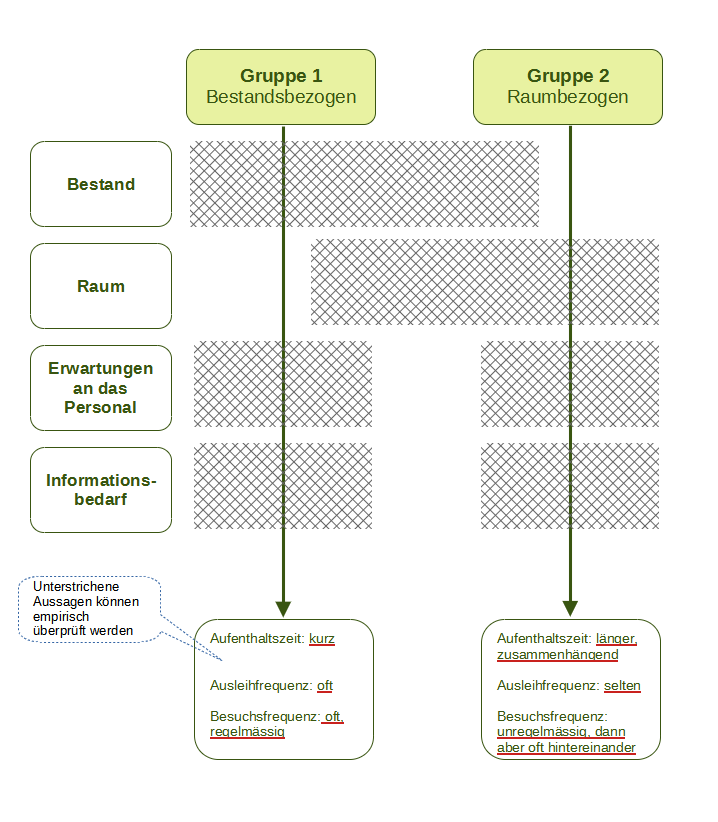
\includegraphics{img/Skizze_Modell.png}
\caption{Abb. 1: Skizze Konzeptuelles Modell}
\end{figure}

\hypertarget{potentielle-forschungsfragen}{%
\section{5. Potentielle
Forschungsfragen}\label{potentielle-forschungsfragen}}

Das präsentierte konzeptionelle Modell sowie die vorhergehende
Diskussion impliziert eine Reihe von Forschungsfragen, die sowohl durch
Forschende -- also solche, die an Einrichtungen wie Hochschulen
angestellt sind, aber zum Beispiel auch Studierende in ihren
Abschlussarbeiten -- als auch durch Personen aus der Bibliothekspraxis
angegangen werden können. Grundsätzlich ist die Forschung für und über
Bibliotheken im DACH-Raum so aufgestellt, dass sie grösstenteils nicht
frei -- im Sinne von ohne Finanzierungsdruck oder finanziert über
Forschungsförderer -- durchgeführt werden kann, sondern eigentlich fast
nur, wenn sie von Bibliotheken finanziert oder im Rahmen der Ausbildung
organisiert wird. Insoweit bietet sich eine, vielleicht auch lose --
also nicht abgesprochene, aber über Publikationen von Ergebnissen von
getrennten Studien miteinander verbundene --, Kooperation von Forschung
und Praxis an.

\begin{enumerate}
\def\labelenumi{\arabic{enumi}.}
\item
  Als erster Punkt stünde an, die Vorhersagen, welche im konzeptionellen
  Modell gemacht wurden, empirisch zu überprüfen und zwar nicht nur in
  einer Bibliothek -- deren Ergebnisse ja immer durch die lokalen
  Umstände bedingt wären -- sondern in möglichst vielen. Hierfür bieten
  sich Umfragen und Beobachtungen explizit an, in denen Aufenthaltsdauer
  und Mediennutzung von Personen in Öffentlichen Bibliotheken erhoben
  werden. Im Idealfall sollten verschieden grosse Bibliotheken, in
  verschiedenartigen -- also vor allem unterschiedlich grossen --
  Gemeinden untersucht werden. Dies würde ermöglichen, nicht nur die
  Voraussagen zu überprüfen, sondern auch, die jeweiligen Ergebnisse zu
  vergleichen. Falls sich die beiden Gruppen tatsächlich «in den Daten
  zeigen», könnte man dann zum Beispiel fragen, ob sie sich in
  unterschiedlich grossen Bibliotheken in unterschiedlichem Masse zeigen
  oder ob bestimmte Angebotsformen wie Bibliothekscafés oder Makerspaces
  einen Unterschied zu machen scheinen. Hilfreich für einen solchen
  weitergehenden Vergleich wäre, wenn für diese empirische Überprüfung
  jeweils die gleichen Messinstrumente, also beispielsweise die gleiche
  Frage- oder Beobachtungsbögen, verwendet würden. Dies könnte erreicht
  werden, indem sie im Vorfeld zwischen verschiedenen Forschenden oder
  Bibliotheken abgestimmt oder aber, indem diese Instrumente offen
  publiziert und dann nachgenutzt werden.
\item
  Eine weiterführende Frage wäre die, ob Bibliothekar*innen diese
  unterschiedlichen Gruppen in ihrer täglichen Arbeit wahrnehmen und
  wenn ja, wie sie auf diese reagieren. Im Kapitel 2 wurde angeführt,
  dass es Hinweise darauf gibt, dass die Arbeit in Bibliotheken zum Teil
  schon so organisiert ist, als wenn dies der Fall wäre. Insoweit könnte
  unter Umständen schon weiterführendes Wissen aus der Praxis erhoben
  werden. Dies wäre wieder vor allem dann sinnvoll, wenn es in mehreren
  unterschiedlichen Bibliotheken getan wird.
\item
  Im Kapitel 3 wurde postuliert, dass das Vorhandensein der beiden
  Gruppen auch bedeuten würde, dass der Einsatz von Ressourcen in
  Bibliotheken und die Bewertung von Bibliotheksarbeit effektiver
  geplant werden könnte. Hilfreich wäre wohl, dies konkreter
  auszuarbeiten, damit die mögliche Bedeutung der These sichtbarer wird.
  Was genau würde sich ändern? Wie genau könnte der Einsatz von
  Personal, die Entwicklung von Angeboten oder die interne Verteilung
  von Aufgaben vorgenommen werden, wenn sich die Existenz der beiden
  Gruppen zeigen liesse?
\item
  Wie in der These angedeutet, ist ein «Wechsel» zwischen diesen Gruppen
  für Menschen möglich. Auch das könnte man untersuchen, beispielsweise
  indem man den Wandel der Bibliotheksnutzung während der
  «Bibliotheksbiographie» von Menschen betrachtet. Sinnvoll wäre dann
  zum Beispiel danach zu fragen, was einen solchen Wechsel bedingt. Ist
  es zum Beispiel so, dass Menschen in einem bestimmten Alter oder in
  einer bestimmten sozialen Situation -- zu denken ist wohl daran, ob
  sie aktuell eine Bildungseinrichtung besuchen oder nicht -- eher zu
  einer der beiden Nutzungsweisen tendieren? Oder ist es eine rein
  individuelle Entscheidung?
\item
  Weiterhin ist das konzeptionelle Modell, auch da es als Beispiel
  gedacht ist, noch relativ einfach. Es wird nur von zwei Gruppen
  ausgegangen. Aber es liesse sich wohl mit guten Gründen weiterführen.
  Man kann gut nach möglichen Differenzierungen innerhalb der beiden
  Gruppen fragen (unter anderem danach, ob Jugendliche der raumbezogenen
  Gruppe grundsätzlich anderes tun als junge Erwachsene oder Personen
  der gleichen Gruppe, die aber aufgrund ihres Alters ausserhalb der
  formalen Bildungssysteme stehen) und man kann fragen, ob es nicht noch
  weitere Gruppen gibt. Dies kann forschend aus zwei Richtungen
  angegangen werden. So liesse sich das Modell mit weiteren Überlegungen
  und Evidenzen theoretisch erweitern und differenzieren. Gleichzeitig
  liesse sich eine Erweiterung aber auch aus empirischen Daten
  herausarbeiten, falls diese erst einmal erhoben würden, um das Modell
  überhaupt -- wie in diesem Kapitel unter Punkt eins erwähnt -- zu
  überprüfen.
\end{enumerate}

\hypertarget{fazit}{%
\section{6. Fazit}\label{fazit}}

In diesem Text wurde dargelegt, wie sich ein soziologisch orientiertes
Denken, das danach fragt, wie Institutionen funktionieren, konkret auf
die Öffentlichen Bibliotheken anwenden lässt. Das erarbeitete
konzeptionelle Modell sollte dabei nicht nur als mögliches Beispiel
verstanden werden, sondern als ernsthafter Beitrag dazu, die konkrete
Arbeit von Bibliotheken zu verstehen.

Aber gleichzeitig ist der Text auch in der Hoffnung geschrieben, dass er
in der bibliothekarischen Praxis und der auf Bibliotheken bezogenen
Forschung in dem Sinne aufgegriffen wird, dass sich weitere solcher
Gedanken gemacht werden. Es gab im Laufe der Bibliotheksgeschichte im
DACH-Raum schon mindestens zweimal -- in den 1920er und 1930er Jahren
und dann noch einmal in den 1970er Jahren -- Ansätze dazu,
soziologisches Denken in das Bibliothekswesen zu integrieren. Beide sind
gewissermassen «ausgelaufen» und wurden jeweils durch ein Denken über
Bibliotheken ersetzt, das recht wenig mit empirischen Daten und
theoretischer Modellierung der Bibliotheksnutzung arbeitet.\footnote{Es
  ist hier nicht der Ort, darüber nachzudenken, warum dies passiert ist.
  Aber eine Durchsicht der bibliothekarischen Zeitschriften aus dem
  DACH-Raum zeigt erstens sehr schnell, dass sich in den 1920er und
  1930er Jahren (inklusive der ersten Jahre des Nationalsozialismus) und
  dann noch einmal in den 1970er Jahren in ihnen verstärkt soziologisch
  orientierte Arbeiten finden, die sich beispielsweise durch die
  Darstellung von empirischen Daten, Strukturdiagrammen und Modellen
  auszeichnen, welche gesellschaftliche Zusammenhänge darzustellen
  versuchen. Vergleichbare Texte finden sich in den anderen Jahrzehnten
  in der deutschsprachigen bibliothekarischen Fachliteratur, die seit
  1900 erschien, fast nicht. Zu vermuten ist aber, dass die
  «Politisierung» der jeweiligen soziologischen Ansätze -- in den 1930er
  Jahren hin zu rassistisch-völkischen Fragestellungen und in den 1970er
  Jahren zu Fragen, wie mit den gesellschaftlichen Antagonismen
  umgegangen werden kann -- damit zu tun hat, dass diese Ansätze später
  nicht mehr aufgegriffen wurden. Es scheint aber, dass dies heute nicht
  mehr der Fall sein muss und deshalb wieder neu soziologisches Denken
  in das Bibliothekswesen integriert werden könnte.} Das hier
dargestellte konzeptionelle Modell hat hoffentlich gezeigt, dass es
weiterhin sinnvoll, möglich und auch vorteilhaft für die Planung der
bibliothekarischen Arbeit sein kann -- neben den intellektuell
anregenden Herausforderungen, die sich stellen -- soziologisch
orientiert über Bibliotheken nachzudenken.

\hypertarget{literatur}{%
\section{Literatur}\label{literatur}}

Allison, Deeann ; DeFrain, Erica ; Hitt, Brianna D. ; Tyler, David C.
(2019). \emph{Academic library as learning space and as collection: A
learning commons' effects on collections and related resources and
services}. In: The Journal of Academic Librarianship 45 (2019) 3:
305--314, \url{https://doi.org/10.1016/j.acalib.2019.04.004}

Cisney, Lori (2023). \emph{Active learning: a consideration in
collection developement in health sciences libraries?} In: Collection
and Curation 42 (2023) 2: 41--45,
\url{https://doi.org/10.1108/CC-02-2022-0009}

Kroski, Ellyssa (edit.) (2020). \emph{Ready-to-use Gaming Programs for
Libraries.} Chicago: ALA Editions, 2020

McMenemy, David ; Robinson, Elaine ; Ruthven, Ian (2022). \emph{The
Impact of COVID-19 Lockdowns on Public Libraries in the UK: Findings
from a National Study}. In: Public Library Quarterly 42 (2023) 1,
\url{https://doi.org/10.1080/01616846.2022.2058860}

Nicholson, Scott (2010). \emph{Everyone Plays at the Library: Creating
Great Gaming Experineces fo All Ages.} Medford: Information Today, 2010

Nicholson, Scott (2013). \emph{Introduction.} In: Library Trends 61
(2013) 4: 751--754,

Redaktion LIBREAS (2022). CfP \#43: Soziologie der Bibliothek. In:
Weblog LIBREAS.Library Ideas, 18.11.2022,
\url{https://libreas.wordpress.com/2022/11/18/cfp-43-soziologie-der-bibliothek/}

Schuldt, Karsten (2022). \emph{Waren Öffentliche Bibliotheken im
DACH-Raum 2020 in einer Krise?: Ein Blick auf die
Bibliotheksstatistiken}. In: Informationspraxis 8 (2002) 1,
\url{https://doi.org/10.11588/ip.2022.1.89240}

%autor
\begin{center}\rule{0.5\linewidth}{0.5pt}\end{center}

\textbf{Dr. Karsten Schuldt}, Wissenschaftlicher Projektleiter am Schweizerischen Institut für Informationswissenschaft, FH Graubünden und Redakteur LIBREAS. Library Ideas.

\end{document}
